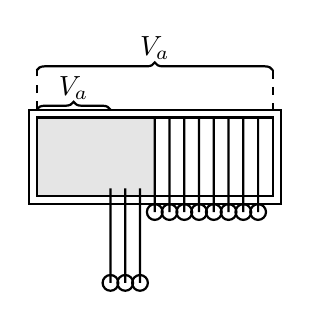
\begin{tikzpicture}[baseline=0.5cm]
  \def\sysLen{3};
  \def\sysHei{1};
  \def\pinRad{0.1};
  \def\pinDis{0.2};
  \def\pinExt{0.9};
  \def\filCol{white!90!black};
  \def\borDis{0.1};
  \def\numPin{7};
  \def\pinLef{3};
  \def\braDis{0.5};
  \def\braAmp{0.1};
  \fill[\filCol] (0,0) rectangle (\sysLen/2,\sysHei);
  \draw[thick] (0,0) rectangle ++(\sysLen,\sysHei);
  \draw[thick] (-\borDis,-\borDis) rectangle (\sysLen+\borDis,\sysHei+\borDis);

  \foreach \x in {1,...,\pinLef} \draw[thick] ({\sysLen/2-\x*\sysLen/2/(\numPin+1)},-\pinDis-\pinExt) circle (\pinRad) to ++(0,\sysHei+\pinDis);

  \draw[thick,decorate,decoration={brace,amplitude=\braAmp cm}] (0,\sysHei+\borDis) to node[above] {$V_a$} ({\sysLen/2-\pinLef*\sysLen/2/(\numPin+1)},\sysHei+\borDis);

  \draw[thick,dashed] (0,\sysHei+\borDis) to ++(0,\braDis);
  \draw[thick,decorate,decoration={brace,amplitude=\braAmp cm}] (0,\sysHei+\borDis+\braDis) to node[above] {$V_a$} ++(\sysLen,0);
  \draw[thick,dashed] (\sysLen,\sysHei+\borDis+\braDis) to ++(0,-\braDis);

  \foreach \x in {0,...,\numPin} \draw[thick] ({\sysLen/2+\x*\sysLen/2/(\numPin+1)},-\pinDis) circle (\pinRad) to ++(0,\sysHei+\pinDis);
\end{tikzpicture}
